
%(BEGIN_QUESTION)
% Copyright 2006, Tony R. Kuphaldt, released under the Creative Commons Attribution License (v 1.0)
% This means you may do almost anything with this work of mine, so long as you give me proper credit

Determine a pair of standard capacitor and resistor values for this op-amp circuit that will produce a 5 volt output voltage signal for an input voltage signal changing at a steady {\it rate} of 5 volts per second.

$$\includegraphics[width=15.5cm]{i01525x01.eps}$$

In other words, design this differentiator circuit to have a {\it time constant} of exactly 1 second.

\underbar{file i01525}
%(END_QUESTION)





%(BEGIN_ANSWER)

I'll let you figure out a pair of component values on your own!  There is no single ``correct'' answer, as an infinite number of $RC$ combinations will yield a time constant $\tau_d$ = 1 second.

%(END_ANSWER)





%(BEGIN_NOTES)

$C$ = 1 $\mu$F and $R$ = 1 M$\Omega$ will work.

%INDEX% Electronics review: differentiator circuit

%(END_NOTES)


